\section{Durchführung}
\label{sec:Durchführung}
Vor Versuchsbeginn werden Radius und Masse der beiden verwendeten Kugeln je drei
mal gemessen. Der Versuchsaufbau ist in Abbildung \ref{fig:skizze} zu sehen.

\begin{figure}
  \centering
  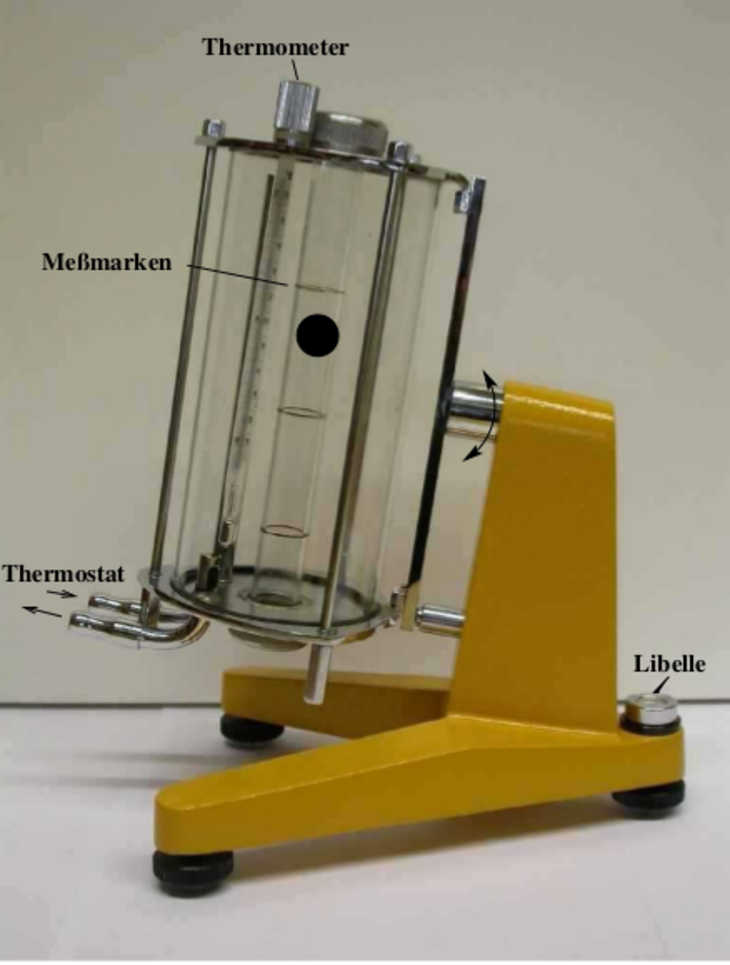
\includegraphics[width=6cm]{bilder/visko.pdf}
  \caption{Viskosimeter \cite{anleitung107}.}
  \label{fig:skizze}
\end{figure}

\noindent Mithilfe der Libelle wird überprüft, ob das Viskosimeter gerade steht.
Ist dies der Fall, wird das innere Rohr mit destilliertem Wasser gefüllt. Dabei
ist darauf zu achten, das sich keine Luftblasen in der Flüssigkeit befinden.
Diese werden eventuell mit einem Glasstab entfernt.
\newline
\newline
Die erste Messung erfolgt bei Raumtemperatur. Die kleinere der beiden Glaskugeln
wird in das Rohr gesteckt,und ihre Fallzeit wird zwischen den drei Meßmarken gemessen,
damit nur die Fallzeit bei konstanter Geschwindigkeit gemessen wird. Erreicht die
Kugel den Boden, wird die Apparatur um $180^\circ$  gedreht. Nachdem 10 Messwerte
aufgenommen sind, wird der gleiche Vorgang mit der größeren Kugel wiederholt.
\newline
\newline
Nun wird das destillierte Wasser erhitzt, und die Fallzeit der großen Kugel gemessen.
Zum Erhitzen wird ein Wasserbad verwendet, welches in ca. $\SI{3}{\celsius}$-Schritten
von $\SI{30}{\celsius}$ auf $\SI{60}{\celsius}$ erwärmt wird. Die aktuelle Temperatur kann mit einem
Thermometer ausgelesen werden. So ergeben sich 10 unterschiedliche Temperaturen,
für die jeweils 2 Werte der Fallzeit notiert werden.
